\documentclass[10pt,aspectratio=43]{beamer}
\usepackage{tikz}
\usetheme{default}
\setbeamertemplate{navigation symbols}{}
\title{Constraint propagation: experiments and bounds}
\subtitle{Generated interaction study}
\author{Research group}
\date{}
\year=2026\month=11\day=5
\newcommand{\fuzzlayerA}[1]{\textbf{#1}}
\newcommand{\fuzzterm}[1]{\fuzzlayerA{#1}}
\newcommand{\fuzzpair}[2]{\fuzzterm{#1}: #2}
\newcommand{\fuzzunit}{ms}
\let\fuzzoriginalunit\fuzzunit
\newcommand{\fuzzcoefficient}{4}
\newcommand{\fuzzscale}[2][\fuzzcoefficient]{#1\,#2}
\definecolor{fuzzpaint}{RGB}{255,0,255}
\definecolor{fuzzsecond}{RGB}{18,137,67}
\tikzset{fuzzvertex/.style={draw,rounded corners=1pt,fill=blue!10,inner sep=1pt,minimum width=.35cm,minimum height=.25cm}}
\begin{document}
\section{Constraint propagation}
\begin{frame}[t,shrink=5]{Constraint propagation}{Composed dependencies}
\fuzzpair{Experiment}{Timing: 12\fuzzunit; estimate $\fuzzscale{x}+\fuzzscale[2]{y}$.}\par
{\renewcommand{\fuzzunit}{samples}\let\fuzzterm\textrm\fuzzpair{LocalScope}{Timing: 7\fuzzunit.}\par}
\fuzzpair{RestoredScope}{Timing: 11\fuzzunit.}\par
\begin{columns}[onlytextwidth,T]
\begin{column}{0.62\textwidth}
\begin{enumerate}
\item {\scriptsize\color{black}\raggedleft
\begin{tabular}{lrr}Method&Cost&Error\\\hline
Local0&21&2\\
Local1&9&18\\
Global2&11&9\\
\end{tabular}\par}
\item \begin{columns}[onlytextwidth,t]
\begin{column}{0.46\textwidth}
\textrm{The next pass} must preserve the boundary conditions while revisiting dependent values. The final diagram records the order in which information crosses the partition. The estimate is $\frac{a+b}{1+c}$.
\end{column}
\begin{column}{0.50\textwidth}
\begin{tabular}{lrr}Method&Cost&Error\\\hline
Cached0&19&13\\
Global1&29&26\\
\end{tabular}
\end{column}
\end{columns}
\item \begin{itemize}
\item \[\begin{pmatrix}a&b\\c&d\end{pmatrix}\begin{pmatrix}x\\y\end{pmatrix}\]
\item \[E=\sum_{i=1}^{n}w_i x_i\]
\item \begin{tabular}{lrr}Method&Cost&Error\\\hline
Global0&19&4\\
Local1&2&29\\
\end{tabular}
\end{itemize}
\end{enumerate}
\end{column}
\begin{column}{0.34\textwidth}
\alt<1-2>{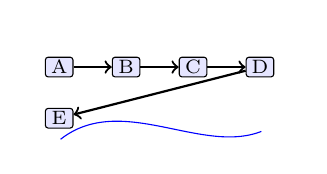
\begin{tikzpicture}[font=\scriptsize]
\begin{scope}[scale=1,rotate=0]
\clip (-.4,-1) rectangle (3.050,.5);

\node[fuzzvertex] (g14n0) at (0.000,0) {A};
\node[fuzzvertex] (g14n1) at (0.850,0) {B};
\node[fuzzvertex] (g14n2) at (1.700,0) {C};
\node[fuzzvertex] (g14n3) at (2.550,0) {D};
\node[fuzzvertex] (g14n4) at (0.000,-0.65) {E};
\begin{scope}[xshift=.5pt,yshift=-.5pt]
\draw<2->[->,thick] (g14n0) -- (g14n1);
\draw<2->[->,thick] (g14n1) -- (g14n2);
\draw<2->[->,thick] (g14n2) -- (g14n3);
\draw<2->[->,thick] (g14n3) -- (g14n4);
\draw[blue] (0,-.9) .. controls (0.765,-.3) and (1.785,-1.1) .. (2.550,-.8);
\end{scope}
\end{scope}
\end{tikzpicture}}{Alternative estimate $x_0$.}
\par
\textbf{We compare the} proposed solution with a reference computed from the complete input.  The estimate is $\frac{a+b}{1+c}$.
\par
\begin{description}
\item<1->[Stage 1] \textrm{A local update} can change the measurements used by several neighboring components.  The estimate is $x_i+x_{i+1}$.
\item<2->[Stage 2] \textit{A local update} can change the measurements used by several neighboring components.  The estimate is $\frac{a+b}{1+c}$.
\item<3->[Stage 3] 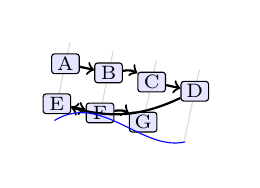
\begin{tikzpicture}[font=\scriptsize]
\begin{scope}[scale=0.8,rotate=-12]
\clip (-.4,-1) rectangle (2.600,.5);
\foreach \x in {0,1,2,3} {\draw[gray!30] (\x*0.700,-.8)--(\x*0.700,.35);}
\node[fuzzvertex] (g19n0) at (0.000,0) {A};
\node[fuzzvertex] (g19n1) at (0.700,0) {B};
\node[fuzzvertex] (g19n2) at (1.400,0) {C};
\node[fuzzvertex] (g19n3) at (2.100,0) {D};
\node[fuzzvertex] (g19n4) at (0.000,-0.65) {E};
\node[fuzzvertex] (g19n5) at (0.700,-0.65) {F};
\node[fuzzvertex] (g19n6) at (1.400,-0.65) {G};
\begin{scope}[xshift=.5pt,yshift=-.5pt]
\draw<2->[->,thick] (g19n0) -- (g19n1);
\draw<2->[->,thick] (g19n1) to[bend left=20] (g19n2);
\draw<2->[->,thick] (g19n2) -- (g19n3);
\draw<2->[->,thick] (g19n3) to[bend left=20] (g19n4);
\draw<2->[->,thick] (g19n4) -- (g19n5);
\draw<2->[->,thick] (g19n5) to[bend left=20] (g19n6);
\draw[blue] (0,-.9) .. controls (0.630,-.3) and (1.470,-1.1) .. (2.100,-.8);
\end{scope}
\end{scope}
\end{tikzpicture}
\end{description}
\par
\begin{block}{Constraint propagation}
\begin{tabular}{lrr}Method&Cost&Error\\\hline
Local0&25&15\\
Cached1&23&21\\
Local2&17&0\\
\end{tabular}
\par
\begin{tabular}{lrr}Method&Cost&Error\\\hline
Global0&14&16\\
Fresh1&0&24\\
\end{tabular}
\par
\textit{The next pass} must preserve the boundary conditions while revisiting dependent values.  The estimate is $\sum_{i=1}^{n}x_i$.
\end{block}
\end{column}
\end{columns}
\par 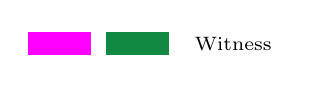
\begin{tikzpicture}[font=\scriptsize]
\fill<2-3>[fuzzpaint] (0,0) rectangle (.8,.3);
\fill<3->[fuzzsecond] (1,0) rectangle (1.8,.3);
\node[anchor=west] at (2,0.15) {Witness};
\end{tikzpicture}
\only<5>{}
\end{frame}
\renewcommand{\fuzzunit}{Hz}
\renewcommand{\fuzzcoefficient}{2}
\renewcommand{\fuzzterm}[1]{{\textit{#1}}}
\section{Message passing}
\begin{frame}[t]{Incremental analysis}
\fuzzpair{MacroStageB}{Timing: 12\fuzzunit, retained: 9\fuzzoriginalunit.}\par
{\renewcommand{\fuzzunit}{local}\fuzzpair{FrameLocal}{Timing: 5\fuzzunit.}\par}
\fuzzpair{FrameRestored}{Timing: 8\fuzzunit; estimate $\fuzzscale{x}$.}\par
\begin{columns}[T]\begin{column}{.46\textwidth}A narrow column can change line breaking even when the underlying expression is unchanged.\end{column}\begin{column}{.46\textwidth}\begin{itemize}\item Input state\item Updated state\end{itemize}\end{column}\end{columns}
\end{frame}
\renewcommand{\fuzzunit}{min}
\renewcommand{\fuzzcoefficient}{3}
\renewcommand{\fuzzterm}[1]{{\textit{#1}}}
\section{Iterative refinement}
\begin{frame}[t]{Cache invalidation}
\fuzzpair{MacroStageC}{Timing: 12\fuzzunit, retained: 9\fuzzoriginalunit.}\par
{\renewcommand{\fuzzunit}{local}\fuzzpair{FrameLocal}{Timing: 5\fuzzunit.}\par}
\fuzzpair{FrameRestored}{Timing: 8\fuzzunit; estimate $\fuzzscale{x}$.}\par
\begin{block}{Follow-up}\fuzzterm{A revised value} depends on the preceding frame.\end{block}
\[r_{k+1}=r_k-\alpha d_k\]
\end{frame}
\renewcommand{\fuzzunit}{us}
\renewcommand{\fuzzcoefficient}{4}
\renewcommand{\fuzzterm}[1]{{\textrm{#1}}}
\section{Message passing}
\begin{frame}[t]{Constraint propagation}
\fuzzpair{MacroStageD}{Timing: 12\fuzzunit, retained: 9\fuzzoriginalunit.}\par
{\renewcommand{\fuzzunit}{local}\fuzzpair{FrameLocal}{Timing: 5\fuzzunit.}\par}
\fuzzpair{FrameRestored}{Timing: 8\fuzzunit; estimate $\fuzzscale{x}$.}\par
\begin{columns}[T]\begin{column}{.46\textwidth}The next pass must preserve the boundary conditions while revisiting dependent values.\end{column}\begin{column}{.46\textwidth}\begin{itemize}\item Input state\item Updated state\end{itemize}\end{column}\end{columns}
\end{frame}
\end{document}
